%!TEX root = main.tex
\section{Neural Networks} \label{sec:prob1}
In this problem, we implement a simple neural network in Python.
The network is trained with backpropogation and stochastic gradient descent.

\subsection{Part 1}
In this problem, we are mainly interested in classification tasks.
Thus, we pass the output of the final hidden layer through a softmax layer to generate a probability (outputs are positive and sum to 1) vector where each element $k$ is the probability of the input being in class $k$.

In general, the training objective is to minimize loss, so at each training step, we evaluate the loss function and compute its gradient, and then adjust the weights and biases in a direction to decrease loss according to the learning rate.
According to the backpropogation algorithm, the derivative of loss with respect to final activation is $\delta^L = Diag[f'(z)] \nabla_a loss$.
For this network with softmax output activation and cross-entropy loss function, we can compute $\delta^L = p(x) - y$, where p(x) is the predicted output for a particular training data point, $x$ in class $y$ (where p is also a function of the network weights, and other parameters).


\subsection{Part 2}
We initialize biases to zero, but we should not initialize weights to zero as well.
This is because with weights of zero, every element of the hidden layer would be the same, since the hidden layer is based on input layer and weights.
If every element of the hidden layer is the same, there is no way to break the symmetry, because backpropogation would consider every weight equally responsible for the network's loss.

Therefore, according to the Xavier Initialization, we can initialize weights to be a zero-mean Gaussian, where the variance is a key parameter.
If variance is too low, all the weights will be close to zero and we will be faced with the same problem described above.
If variance is too high, training the network will take a long time to undo the bias imposed during initialization.
Even worse, it's possible the network will get stuck in a local minimum that is far from the global optimum.
This tradeoff of initializing enough randomness to avoid symmetry while not imposing too much bias, is an important piece of neural network training.
The recommended variance is $\frac{1}{n}$, where $n$ is the number of inputs to that layer.

\subsection{Part 3}
To add weight regularization, the objective function would look like:
\begin{equation}
J(w) = l(w) + \lambda(||w^{(1)}||^2_F + ||w^{(2)}||^2_F)
\end{equation}
The only change to the pseudo-code from the lecture notes would be an updated gradient term during the output layer's backpropogation step.

The effect of regularization on the network would be the same as regularization in general.
The $\lambda$ term penalizes weight matrix size, so increasing $\lambda$ causes weight matrices to shrink in size (lower model complexity), which decreases training accuracy (less likely to overfit), but should increase test accuracy, up to a point where $\lambda$ is large enough that the weight term dominates the loss term in the objective function.


\subsection{Part 4}
Next, we use the network for binary classification on the 2D datasets from the previous homework assignment.

\begin{table}[ht!]
\centering
\begin{tabular}{||c c c c c c c c c||}  
 \hline
 \multirow{2}{*}{Dataset} &
       \multicolumn{2}{c}{1 HL (sm)} &
       \multicolumn{2}{c}{1 HL (lg)} &
       \multicolumn{2}{c}{2 HL (sm)} &
       \multicolumn{2}{c||}{2 HL (lg)} \\
 & Train & Test & Train & Test & Train & Test & Train & Test \\ [0.5ex] 
 \hline\hline
 1 & 100.0 & 99.5 & 99.8 & 99.5 & 100.0 & 100.0 & 100.0 & 100.0 \\ \hline
 2 & 94.5 & 91.5 & 95.25 & 93.0 & 94.5 & 91.5 & 95.0 & 94.5 \\ \hline
 3 & 98.5 & 95.0 & 98.25 & 96.5 & 98.25 & 96.0 & 98.0 & 96.0 \\ \hline
 4 & 96.25 & 95.25 & 97.0 & 94.0 & 95.25 & 93.75 & 93.75 & 92.50 \\ \hline
\end{tabular}
\caption{Accuracy of NN on 2D datasets.}
\label{table_1_4}
\end{table}

The results in \cref{table_1_4} show the training and test accuracy for four 2D datasets, with four different network architectures (1 or 2 hidden layers (HL) and small or large number of hidden nodes).
The accuracies in general are quite high ($>90\%$).
As expected, test accuracy is worse than training accuracy for almost all cases.
Training was terminated after the change in validation loss from the previous epoch was small, which is one method to protect against overfitting.

An example of how the decision boundary changes with architecture is shown in~\cref{fig:1_4_arch}.
The simpler model~\cref{fig:arch_init1} leads to a simpler decision boundary (somewhat more linear) than the complex model~\cref{fig:arch_init2}

\begin{figure}
\centering
\begin{subfigure}{.25\textwidth}
  \centering
  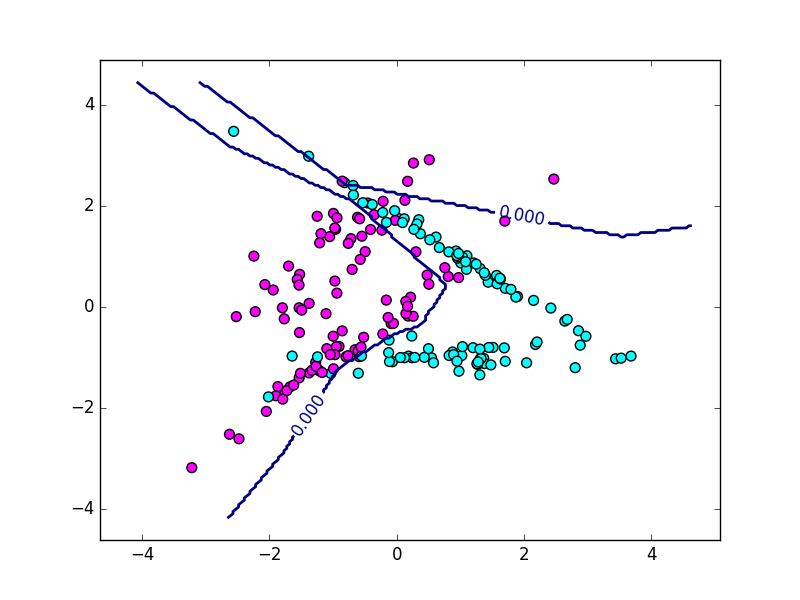
\includegraphics[width=.9\linewidth]{figures/1_4_data2_1hl_small}
  \caption{1 Hidden Layer (small)}
  \label{fig:arch_init1}
\end{subfigure}%
\begin{subfigure}{.25\textwidth}
  \centering
  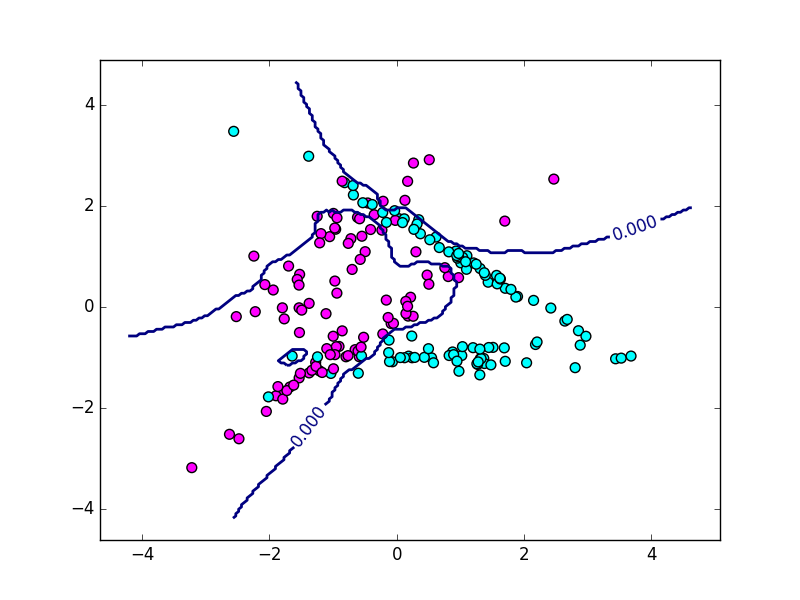
\includegraphics[width=.9\linewidth]{figures/1_4_data2_2hl_large}
  \caption{2 Hidden Layers (large)}
  \label{fig:arch_init2}
\end{subfigure}
\caption{The low-complexity model (left) with one small hidden layer (10 nodes) has a simpler decision boundary than the high-complexity model (right) with two large hidden layers (100 nodes each).}
\label{fig:1_4_arch}
\end{figure}

A thorough hyperparameter search could be done for this problem to find optimal learning rate, but a value around $10^{-3} - 10^{-4}$ worked well for most scenarios.

It is worth noting the effect of initialization, as depicted in \cref{fig:init}.
Since the weights are initialized randomly, sometimes the network would not converge to a good decision boundary (\cref{fig:sub_init1}~vs.~\cref{fig:sub_init2}), and the boundaries varied significantly from run-to-run.
This makes it less meaningful to compare architectures with results from single runs.

\begin{figure}
\centering
\begin{subfigure}{.25\textwidth}
  \centering
  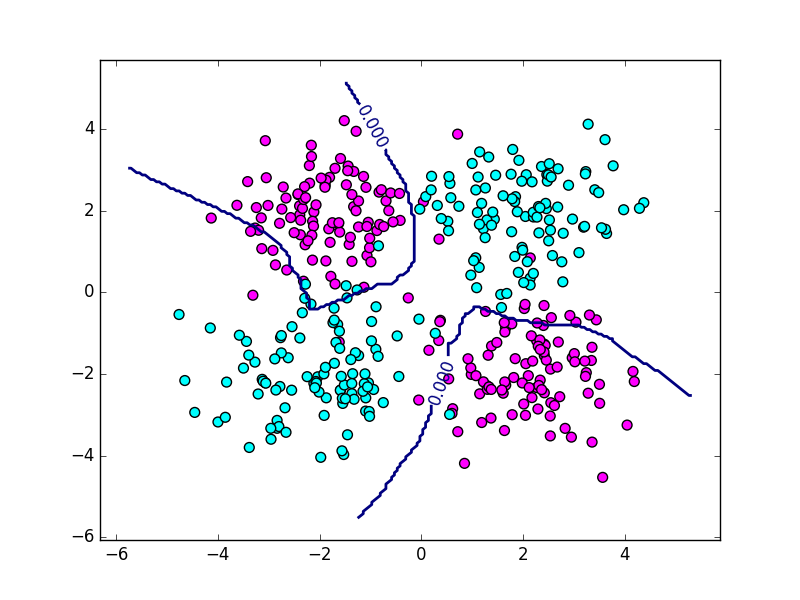
\includegraphics[width=.9\linewidth]{figures/1_4_data4_2hl_large_good}
  \caption{Good initialization}
  \label{fig:sub_init1}
\end{subfigure}%
\begin{subfigure}{.25\textwidth}
  \centering
  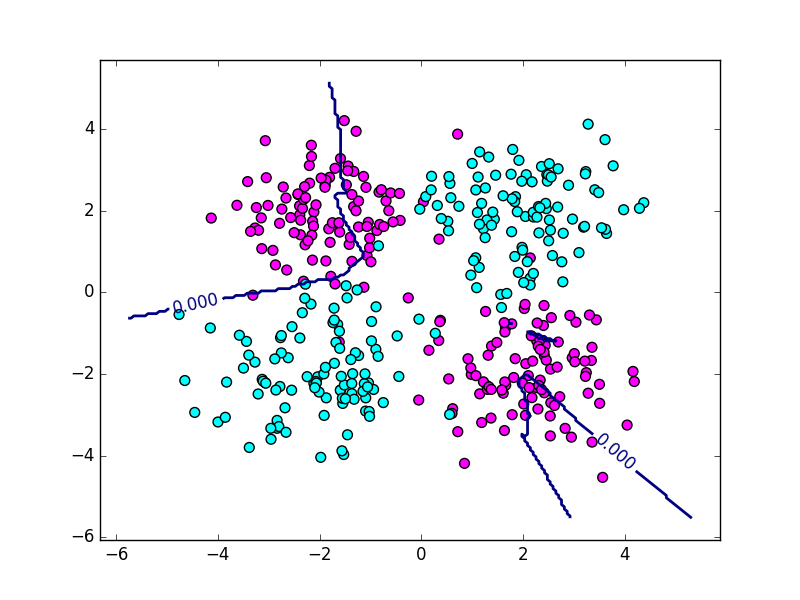
\includegraphics[width=.9\linewidth]{figures/1_4_data4_2hl_large_bad}
  \caption{Bad initialization}
  \label{fig:sub_init2}
\end{subfigure}
\caption{The random initialization has a large effect on final decision boundary. On the left, the boundary is pretty good. The boundary on the right is much worse even with all the same hyperparameters and model structure.}
\label{fig:init}
\end{figure}

In general, the NN classifier works best on the (easy) linearly separable dataset ($\approx 100\%$ on 1), and still does very well on the other datasets with non-linear decision boundaries.

Compared to the classifiers from the previous homework assignment, the NN of course outperforms Linear SVM and LR on the non-linearly separable data, and does approximately as well on the linearly separable ones. The performance is also comparable/better than Guassian RBF SVM and training time seems much faster (though speed depends on quality of implementation).

\subsection{Part 5}
Finally, we use the network for digit classification on the MNIST dataset.
Results are shown in~\cref{fig:1_5_acc}, where the training accuracy is 98\% and validation accuracy is 86\%.
This performance is very good, and training takes $<1$ min on a CPU.

The model used was a NN with a single hidden layer with 100 elements.
The accuracy was lower with a smaller number of nodes.

Learning rate was $10^{-2}$, which was chosen by trying multiple values and choosing the one with best validation accuracy.
When learning rate was too high ($>0.1$), learning diverged and some weights became NaN.
Accuracy was similar with learning rate $10^{-2} - 10^{-4}$
When learning rate was too low ($<10^{-6}$), learning was extremely slow ($<30\%$ accuracy after 100 epochs).

Normalization is imporant for this dataset, as our network was unable to converge without first normalizing the data to be within [-1,1].

\begin{figure}
	\centering
	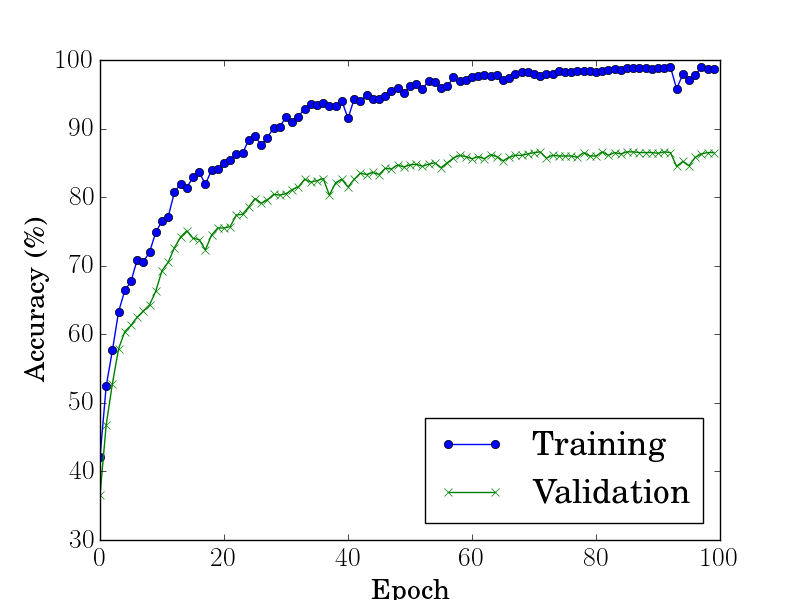
\includegraphics [trim=0 0 0 0, clip, angle=0, width=0.8\columnwidth,
	keepaspectratio]{figures/1_5_acc}
	\caption{For digit classification on MNIST dataset, training and validation accuracy are plotted over 100 epochs. Training accuracy is better than validation accuracy (as expected), and they level out around 98\% and 86\%, respectively.} 
	\label{fig:1_5_acc} 
\end{figure}


